
\documentclass[a4paper,fleqn]{cas-sc}

\usepackage{float}
\usepackage[utf8]{inputenc}
\usepackage[numbers]{natbib}
\usepackage{tabularx}
\usepackage[english]{babel}
\usepackage{amsmath}
\usepackage{amsfonts}
\usepackage{amssymb}
\usepackage{booktabs}
\usepackage{multirow}
\usepackage{hyperref}
\usepackage{subcaption}
\usepackage{color}
\usepackage{xcolor}
\usepackage{lineno}
\usepackage[htt]{hyphenat}
\setlength{\emergencystretch}{2em}
% Keep the float-heavy manuscript inside the journal page budget.
\setlength{\textfloatsep}{8pt plus 2pt minus 2pt}
\setlength{\floatsep}{8pt plus 2pt minus 2pt}
\setlength{\intextsep}{8pt plus 2pt minus 2pt}
\setlength{\bibsep}{2pt plus 0.5pt minus 0.5pt}

% Preprint footer: drop the "submitted to Elsevier" wording.
\ExplSyntaxOn
\cs_set:Npn \__first_footerline:
  {
    \group_begin:
    \small
    \sffamily
    \ifnum\theblind>0\relax
    \else
    \__short_authors: :~
    \fi
    \rmfamily \itshape Preprint
    \group_end:
  }
\ExplSyntaxOff
% No ORCID identifiers are used, so hide the empty ORCID footnote.
\RenewDocumentCommand \printorcid { } { }
% The CAS class draws email/URL icons from a thumbnails/ folder. Uploads that
% do not carry that folder fail with "File `thumbnails/cas-email.jpeg' not
% found" and the author footnote breaks. The class has a no-logo mode, so the
% email footnote prints as plain text and the document needs no image assets.
\ExplSyntaxOn
\bool_gset_true:N \g_stm_nologo_bool
\ExplSyntaxOff
%%%Author definitions
\def\tsc#1{\csdef{#1}{\textsc{\lowercase{#1}}\xspace}}
%%%

% Figures and screenshots ship inside Journal_Paper/. The extra prefixes keep
% the build working when the project root is the repository root (or when the
% upload keeps the Journal_Paper/ folder name) instead of Journal_Paper/.
\graphicspath{{./figures/}{./screenshots/}{Journal_Paper/figures/}{Journal_Paper/screenshots/}{../Journal_Paper/figures/}{../Journal_Paper/screenshots/}{../artifacts/figures/}}

\begin{document}
\let\WriteBookmarks\relax
\def\floatpagepagefraction{1}
\def\textpagefraction{.001}

% Short title
\shorttitle{Evidence-Consistent XGBoost}

% Short author
\shortauthors{Rahaman et~al.}

% Main title of the paper
\title [mode = title]{Evidence-Consistent XGBoost for Calibrated Hallucination Risk Estimation in Black-Box Language Model Answers}

% First author and corresponding author
\author[1]{Md. Atikur Rahaman}
\cormark[1]
\ead{mrahaman2310298@bscse.uiu.ac.bd}
\credit{Conceptualization, Methodology, Software, Writing - original draft}

% Second author
\author[1]{Saiful Alam Sabbir}
\ead{sabbir2310105@bscse.uiu.ac.bd}
\credit{Data curation, Investigation, Validation, Visualization}

% Third author
\author[1]{MD. Miraz Ahamed}
\ead{mahamed2310524@bscse.uiu.ac.bd}
\credit{Software, Formal analysis, Writing - review \& editing}

% Supervisor
\author[1]{Ohidujjaman Tuhin}
\credit{Supervision, Validation, Writing - review \& editing}

% Address/affiliation
\affiliation[1]{organization={Computer Science and Engineering, United International University},
  city={Dhaka},
  citysep={},
  postcode={1212},
  country={Bangladesh}}

\cortext[cor1]{Corresponding author: Md. Atikur Rahaman}

% Abstract
\linenumbers
\begin{abstract}
  Large language models answer in fluent text, and some answers are not supported by the evidence that is available. A confidently wrong answer can mislead users in question answering and content review. Current detectors have limits. Judge models are slow and costly. Encoder classifiers need model weights and a GPU. Feature-based systems rarely report calibration or cross-domain results. This study presents a lightweight black-box model that estimates hallucination risk, $P(\text{hallucinated}\mid q, c, a)$, from a question, a reference context, and a candidate answer. The model is called evidence-consistent XGBoost, or EC-XGB. It combines the 26 evidence-consistency features in seven groups with eight claim-level NLI aggregates, so the risk score sees both whole-answer signals and per-claim support statistics. Three changes separate EC-XGB from a standard tuned XGBoost. Length features are log-scaled and monotone constraints tie the risk to the evidence direction, the claim-level aggregates enter the feature vector, and RAGTruth non-QA responses join the training data with a source indicator. Every experiment runs on a grouped 70/15/15 split with seeds 42, 123, and 456, and group-aware splits keep both answer variants of a question in one partition. On HaluEval QA (20{,}000 rows), EC-XGB reaches F1 = 0.9858 and AUROC = 0.9985, on par with the standard model on a saturated benchmark. The gain appears under domain shift. The standard model flags 99.9\% of natural RAGTruth answers as risky, while EC-XGB flags 61.3\%, raises the AUROC from 0.475 to 0.573, and lowers the ECE from 0.635 to 0.283. A display calibrator fitted on RAGTruth QA cuts the deployed ECE from 0.735 to 0.126. An operating-point mode selects the validation threshold for a five percent false-positive budget, and the test recall stays above 99\%. On FaithBench the flag rate falls from 99.5\% to 7.2\% with a higher AUROC, and the conservative F1 drop in that regime is reported as a limitation. One analysis takes 61.8~ms and costs near \$0.001 per 1{,}000 predictions, about 100 times less than the measured LLM judge. A FastAPI service and a Next.js dashboard deploy the model with claim-level evidence checks.
\end{abstract}

% Keywords
% Each keyword is separated by \sep
\begin{keywords}
  Hallucination risk estimation \sep Explainable AI \sep Probability calibration \sep Distribution shift \sep Evidence-consistent XGBoost \sep SHAP
\end{keywords}

\maketitle
\linenumbers

\section{Introduction}\label{sec:intro}

Hallucination detection is an active research area. SelfCheckGPT samples multiple responses and measures their consistency without an external database \cite{selfcheck}. Luna uses a small evaluation model that costs less than a large judge \cite{luna}. Semantic entropy groups sampled answers by meaning and flags confabulation from disagreement, again with no external knowledge \cite{farquhar2024semantic}. A hybrid framework combines frozen encoder features with lightweight classifiers and reports strong benchmark scores \cite{ieeeTai}. Two practical problems remain. Judge models are slow and expensive, and encoder models are hard to interpret. Feature-based detectors are cheaper, but their probabilities are rarely calibrated and their behavior outside the training domain is rarely tested. Two recent surveys group these families and list evaluation and reliability limits among the open questions \cite{huang2025survey,alansari2026survey}. This study builds a black-box model that reads a question, a reference context, and a candidate answer and estimates $P(\text{hallucinated}\mid q,c,a)$. The model, evidence-consistent XGBoost (EC-XGB), combines 26 evidence-consistency features in seven groups with eight claim-level NLI aggregates and a tuned XGBoost classifier, with Platt and isotonic calibration and SHAP explanations. HaluEval QA provides the training and in-domain test data. RAGTruth supplies natural responses for the transfer, multi-source training, and recalibration checks, and FaithBench adds a summarization stress test.

Six recent studies are closest to this work. HaluAgent shows that small language models can select tools and detect multiple hallucination types, yet each answer needs multiple tool calls \cite{haluagent}. Valentin et al. report a calibrated multi-scoring detector with a clear cost analysis, and the detector still depends on LLM scoring for its main signal \cite{costeff}. Sundaragiri et al. combine retrieval grounding, NLI verification, and an XGBoost classifier, and their evaluation reports classification metrics only \cite{ijert}. Haq et al. score hallucination with token-level SHAP-LIME attributions, without testing whether those attributions stay stable \cite{multimedia}. Deng et al. study cross-domain detection and show that detectors lose accuracy outside their training domain, and their method targets multi-turn dialogue signals \cite{spikescore}. FaithBench reports that modern LLMs still produce hard summarization hallucinations, and it is a summarization benchmark with no risk-calibration study \cite{faithbench}.

Four issues remain open in the literature. Calibration is not reported for lightweight detectors, explanation quality is not measured, cross-domain behavior is not tested, and error patterns are not analyzed case by case. This study addresses the four issues together. Group-aware splits and artifact-control baselines cover the benchmark shortcuts, and validation-only calibration answers the reliability question. Zero-shot runs on RAGTruth and FaithBench measure the transfer limits. HaluEval QA is suitable for training because it provides paired correct and hallucinated answers for 10{,}000 questions, and RAGTruth provides natural responses with human span annotations for an external check. The accepted outcomes are a calibrated risk model (EC-XGB) with F1 = 0.9858 on HaluEval QA, a shift result where the flag rate on natural RAGTruth answers falls from 99.9\% to 61.3\% while the AUROC rises from 0.475 to 0.573, a target recalibration that reduces the RAGTruth QA ECE from 0.8185 to 0.1335, an operating point that maximizes recall under a five percent false-positive budget, and a deployed system that completes one analysis in 61.8~ms for near \$0.001 per 1{,}000 predictions.

\section{Conventional Method}\label{sec:conventional}

\subsection{Preliminaries}

A hallucination is text that is fluent but not supported by the available evidence, and detection quality is usually judged with labeled benchmark splits, precision, recall, F1, and AUROC. Two evaluation choices matter for deployment. The first is calibration, since a risk score is only useful when its numeric value matches the observed frequency of hallucinated answers, and expected calibration error and reliability diagrams expose the gap between the two \cite{guo}. The second is interpretability, since a user who sees a high-risk flag needs to know which evidence signal produced it, and feature-attribution methods such as SHAP provide that view for tabular models \cite{shap}. The present work evaluates both properties in a black-box setting, where the detector reads the question, an optional reference context, and the candidate answer, and never inspects the generating model.

\subsection{Existing Methods}

Hallucination detection is an active research area, and the existing methods fall into three broad families: asking a language model to evaluate output consistency, training neural classifiers over frozen encoders, and building on hand-crafted features and interpretable models. Recent surveys organize the same families in more detail and collect their open problems \cite{huang2025survey,alansari2026survey}. LLM-based detection relies on model-internal signals or on a separate judge model. SelfCheckGPT \cite{selfcheck} samples multiple responses and treats their agreement as a hallucination signal, and HaluAgent \cite{haluagent} shows that small language models can act as cheaper detectors. Semantic entropy measures uncertainty over the meaning of those samples instead of their surface form \cite{farquhar2024semantic}. Luna \cite{luna} takes the judge idea further with a lightweight evaluation model that matches larger judges at a fraction of the cost, and a calibrated multi-scoring detector reaches competitive accuracy with an explicit cost analysis \cite{costeff}. None of these judge verdicts gives a feature-level reason, which makes a single failure hard to debug.

A second line of work trains classifiers on top of pretrained encoders, and a hybrid framework in \cite{ieeeTai} combines encoder features with lightweight models and reports strong results on hallucination benchmarks. These methods are accurate, but they need the encoder weights, they run on GPUs, and their embeddings are not directly interpretable. The third family keeps the pipeline interpretable by construction. A multi-signal framework in \cite{ijert} combines retrieval grounding, NLI verification, and an XGBoost classifier, and \cite{multimedia} scores hallucination with token-level SHAP-LIME attributions. Small verifier models such as MiniCheck reach high fact-checking accuracy at low cost, which shows that verification does not always need a large judge \cite{minicheck2024}. The present work differs from \cite{multimedia} in an important way, since it explains predictions at the level of semantically meaningful evidence-consistency features rather than raw tokens, and it adds calibrated risk scores and a cross-domain evaluation that both papers lack.

On the benchmark side, HaluEval \cite{haluEval} and TruthfulQA \cite{truthqa} are standard test beds, FActScore \cite{factscore} measures factual precision in long-form generation, and RAGTruth \cite{ragtruth} contributes naturally generated responses with human word-level annotations that are closer to production data. FaithBench \cite{faithbench} shows that current detectors still struggle on challenging modern-LLM outputs, and SpikeScore \cite{spikescore} demonstrates that cross-domain generalization remains an open problem.

\subsection{Research Gap}

Prior work has explored hallucination detection, feature engineering, calibration, and SHAP in isolation. Three gaps remain open. First, token-level attributions in \cite{multimedia} explain raw text rather than semantically meaningful evidence signals, and the attributions are visualized without any reliability measurement. Second, calibration is rarely reported for lightweight detectors, and target-domain behavior is rarely tested, while the closest multi-signal framework \cite{ijert} reports classification metrics only. Third, the benchmark itself imposes limits, since around 85\% of HaluEval is generated with a sampling-then-filtering procedure \cite{bang-etal-2025-hallulens}, and such data blurs the line between factually wrong and hallucinated content. Cross-domain evaluation remains open as well, and SpikeScore \cite{spikescore} shows that detectors trained in one domain lose accuracy in another. This study fills these gaps by fusing claim-level evidence signals and multitask training into an evidence-consistent XGBoost and by testing calibrated, explainable risk prediction under domain shift with a reproducible artifact.

\section{Proposed Method}\label{sec:proposed}

Figure~\ref{fig:pipeline} shows the full proposed pipeline at a glance. The system takes a question, an optional reference context, and a candidate answer produced by a black-box LLM, and it returns a calibrated risk probability together with per-feature explanations. Each stage is described in the following subsections.

\begin{figure}[pos=htbp]
  \centering
  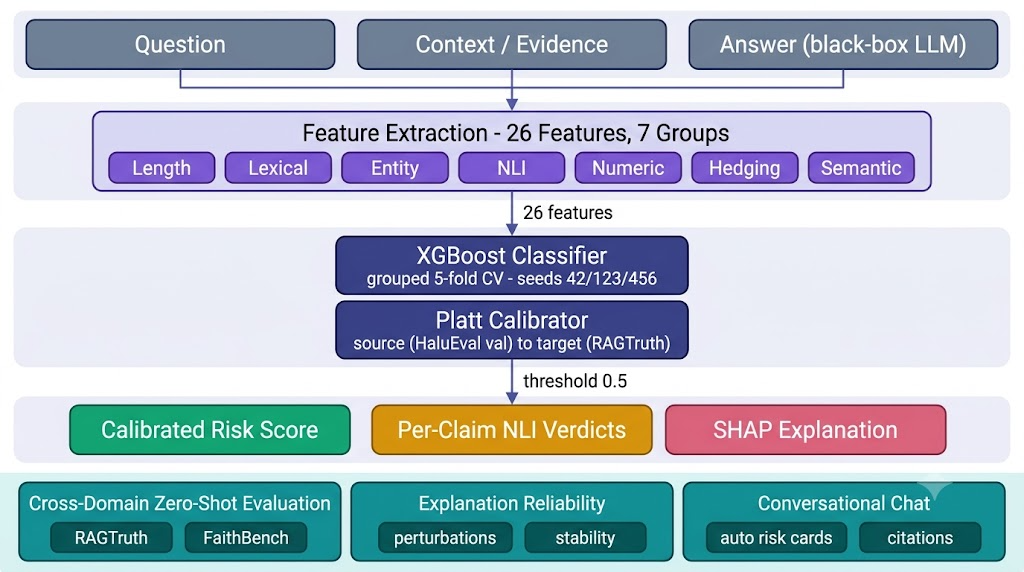
\includegraphics[width=\linewidth]{architecture.png}
  \caption{End-to-end pipeline of the proposed model. Evidence-consistency features from the question, context, and answer feed a grouped-CV trained, Platt-calibrated XGBoost model. Outputs include a calibrated risk score, per-claim NLI verdicts, and SHAP explanations, with cross-domain and explanation-reliability evaluation.}
  \label{fig:pipeline}
\end{figure}

\subsection{Task Definition}

Given a question $q$, an optional reference context $c$ (evidence), and a candidate answer $a$ produced by a black-box LLM, the task is to predict the probability $P(\text{hallucinated} \mid q, c, a)$. The proposed model predicts risk, not truth. It flags answers that are unsupported by, or contradictory to, the available evidence.

\subsection{Features}

Table~\ref{tab:features} lists the 26 base features in seven groups, and Table~\ref{tab:claim} lists the eight claim-level aggregates that the proposed model adds. NLI signals come from a DeBERTa-v3 cross-encoder \cite{deberta} trained on SNLI \cite{snli} and MultiNLI \cite{mnli}, evaluated in both directions, context-to-answer and answer-to-context, which yields six probability features. Semantic similarity uses MiniLM sentence embeddings \cite{sbert,minilm}, entity features use spaCy NER \cite{spacy}, and the numeric and hedging groups are collected with regular expressions and a small hedging lexicon.

\begin{table}[pos=htbp]
  \centering
  \caption{Base feature groups (26 features total).}
  \label{tab:features}
  \begin{tabular}{|p{2.1cm}|p{4.6cm}|p{4.4cm}|}
    \hline
    \textbf{Group} & \textbf{Features}                                   & \textbf{Source}   \\
    \hline
    Length/style   & n\_chars, n\_words, n\_sentences, avg\_word\_len    & regex             \\
    \hline
    Lexical        & overlap vs.\ context \& question, Jaccard $\times$2 & token sets        \\
    \hline
    Entity         & entity counts, overlap ratio, novel-entity ratio    & spaCy NER         \\
    \hline
    NLI            & entail/contradict/neutral $\times$ 2 directions     & cross-encoder NLI \\
    \hline
    Numeric        & number counts, overlap ratio, novel numbers         & regex             \\
    \hline
    Hedging        & hedge count, hedge density                          & lexicon           \\
    \hline
    Semantic       & cosine(context,answer), cosine(question,answer)     & MiniLM            \\
    \hline
  \end{tabular}
\end{table}

\begin{table}[pos=htbp]
  \centering
  \caption{Claim-level NLI aggregates (8 features). The answer is split into at most six claims, each claim is scored against its four best-matching context sentences, and the pair probabilities are aggregated with the same 0.5 cutoffs that the verification layer uses.}
  \label{tab:claim}
  \begin{tabular}{|p{2.3cm}|p{7.0cm}|p{2.9cm}|}
    \hline
    \textbf{Signal} & \textbf{Features} & \textbf{Source} \\
    \hline
    Contradiction   & max and mean contradiction, contradicted-claim ratio & NLI cross-encoder \\
    \hline
    Support         & supported-claim ratio, unsupported-claim ratio, min and mean entailment & NLI cross-encoder \\
    \hline
    Decomposition   & number of claims & sentence splitter \\
    \hline
  \end{tabular}
\end{table}

\subsection{Models}

Eight models are compared. The overlap heuristic sets risk to one minus the lexical overlap between the answer and the context, and its threshold is tuned on validation. Logistic regression on standardized features and a random forest with 300 trees are the two standard classifiers. The standard classifier is XGBoost \cite{xgboost}, trained on the 26 base features, and it serves as the reference for the modified model described next. Three controls isolate the value of the feature design, an NLI-only logistic regression that sees only the six NLI probabilities, an answer-only TF-IDF linear model, and a TF-IDF linear model over the full input. A majority baseline that predicts the negative class for every row confirms the balance of the labels. XGBoost hyperparameters come from a randomized search of 30 iterations over depth, learning rate, tree count, subsample, and column subsampling, scored with 5-fold stratified cross-validation on the training split. The best configuration is depth 4, learning rate 0.01, 500 trees, subsample 0.9, and column subsampling 0.7, with a cross-validated AUROC of 0.9970. Every experiment is repeated with seeds 42, 123, and 456, and results are reported as the mean over seeds.

\subsection{Evidence-Consistent XGBoost}

EC-XGB keeps the standard XGBoost learner and changes three things, added cumulatively so that each change can be measured on its own. The first change replaces the raw length counts with log-scaled values and adds monotone constraints, so risk cannot fall when contradiction or novelty rises and cannot climb when entailment, overlap, or semantic similarity rises. The second change appends the eight claim-level aggregates from Table~\ref{tab:claim}, which lets the classifier see the same evidence signals that the deployed verification layer reports. The third change adds RAGTruth summarization and data-to-text training rows with a binary source indicator, while every RAGTruth QA row stays out of training, which keeps the QA transfer result zero-shot for the multitask model. The deployed checkpoint combines all three changes and is called EC-XGB. A strict decision mode selects the validation threshold whose false-positive rate stays at or below five percent, and the calibration protocol below fits its display score.

\subsection{Calibration}

Calibrators are fit on the validation split only. Platt scaling fits a sigmoid to the raw scores \cite{platt}, and isotonic regression fits a step function \cite{isotonic}, and both are compared against the raw model on the test split with expected calibration error over 10 bins \cite{guo}, Brier score, and reliability diagrams. A second step targets a new domain. When a small labeled sample of the target corpus is available, the calibrator is re-fit on that sample, and the effect is measured on a disjoint held-out part of the target corpus. The deployed EC-XGB display score follows the same rule: its calibrator is fitted on the designated RAGTruth QA calibration split, and the source indicator is set to one for natural responses, the same convention used in the shift evaluation.

\subsection{Explainability and Reliability}

Global interpretability comes from SHAP \cite{shap}. A TreeExplainer over the raw XGBoost model produces mean absolute SHAP importance and beeswarm summaries, and local explanations show the feature contributions behind a single verdict. Explanation reliability is measured directly in this work. Each test answer is perturbed in six ways, by replacing entities, numbers, or dates, removing supporting context, inserting irrelevant context, and shuffling clauses, and the calibrated score should stay stable under neutral perturbations and react to semantic ones. Stability is quantified with Spearman and Kendall rank correlation between the original and perturbed scores, the fraction of top-1 flips, and the top-$k$ Jaccard overlap of the SHAP feature rankings.

\subsection{System Implementation}

The methods above are deployed as a two-tier web application, and Figure~\ref{fig:arch} shows the architecture. The Next.js frontend streams an LLM conversation on the chat page using the assistant-ui library, and the FastAPI backend holds the model, the calibrator, the SHAP explainer, and the feature models, all loaded once at startup. Every machine-learning request from the frontend goes through a backend-for-frontend proxy in the Next.js layer to the FastAPI endpoints, which avoids cross-origin issues and keeps the API key on the server side.

\begin{figure}[pos=htbp]
  \centering
  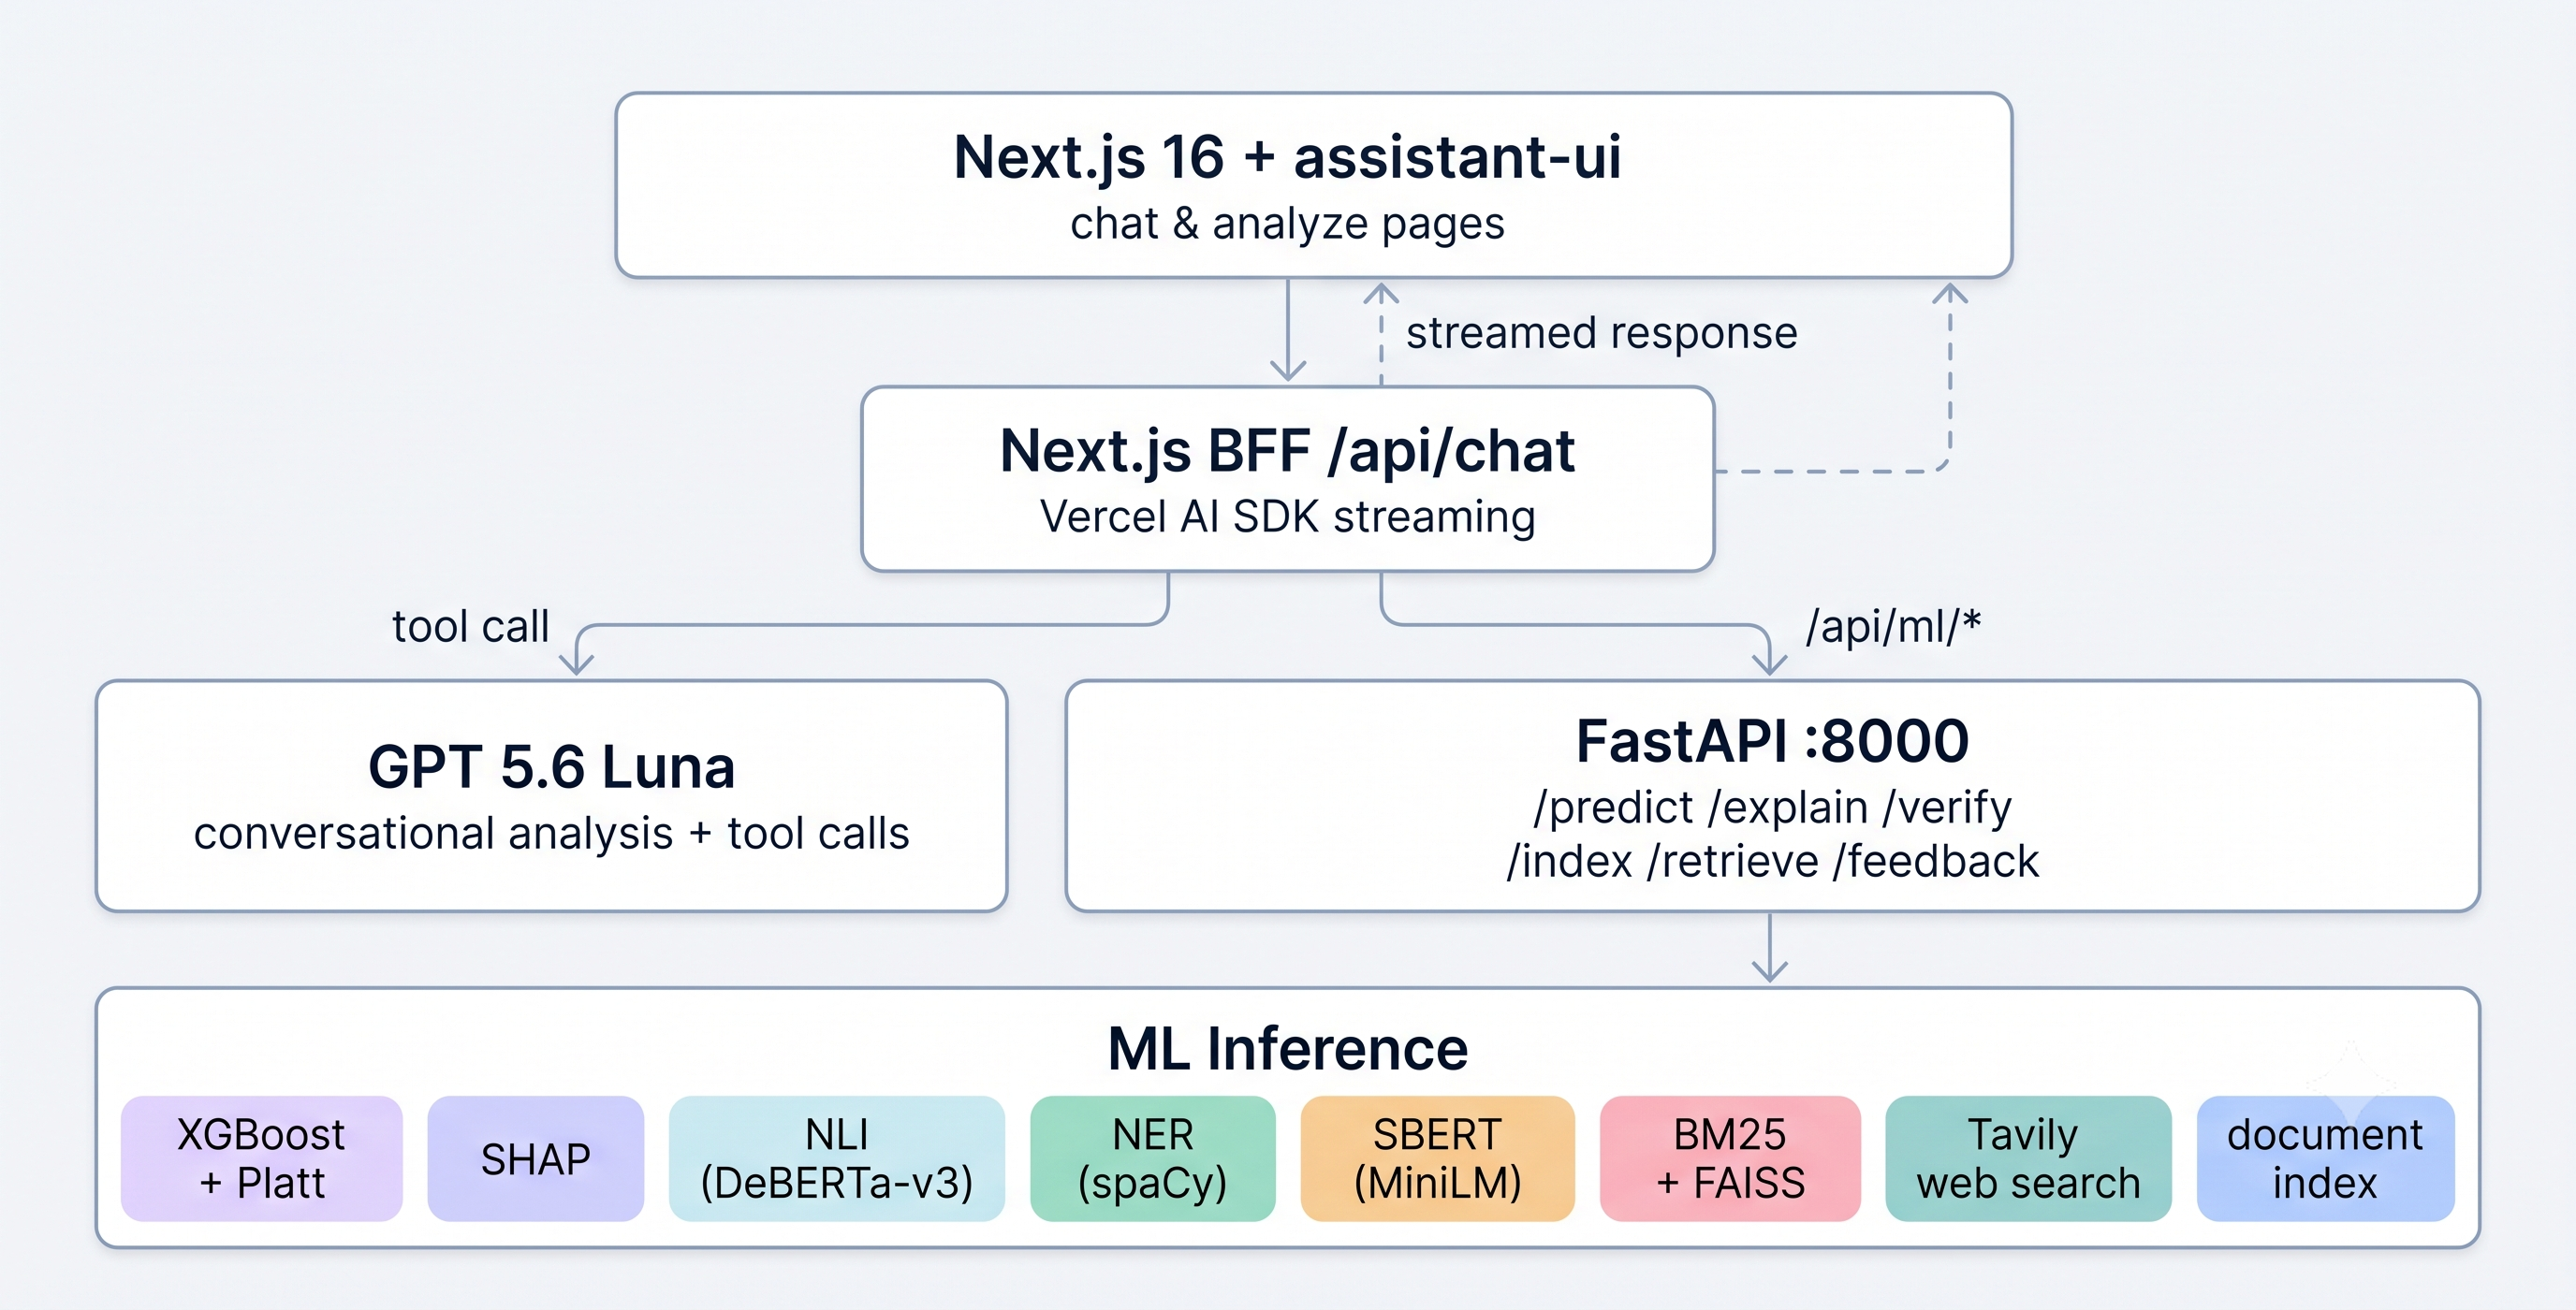
\includegraphics[width=\linewidth]{system_architecture.png}
  \caption{System architecture of the proposed model. The Next.js backend-for-frontend proxies machine-learning requests to FastAPI and streams LLM chat with tool-generated UI widgets.}
  \label{fig:arch}
\end{figure}

The chat page streams through the Vercel AI SDK route. A tool call from the conversation model triggers the analysis endpoint, and the result renders as a risk card inside the message thread with the calibrated score, the per-claim verdicts, the SHAP bars, and an evidence panel that expands the supporting and contradicting passages.

Beyond the score, the system verifies the answer claim by claim. Each claim is decomposed from the answer text and checked with sentence-level NLI against one of three evidence sources, the provided context, an indexed document collection, or live web search. The verdicts supported, contradicted, and unsupported are rendered per claim, with the driving evidence sentence quoted for contradicted claims. Web search uses the Brave Search API with its LLM-context endpoint, and the document index combines BM25, FAISS dense retrieval, and reciprocal rank fusion with a cross-encoder reranker. When the verification score falls into an uncertain band, the claim is routed to an LLM judge that returns a verdict with a short reasoning note.

The verdict headline leads the card. Any contradicted claim sets the risk to high, an unsupported claim sets it to medium, and fully supported claims set it to low, while the standard XGBoost score appears beneath it as the legacy model score. This ordering follows the style-sensitivity result in Section~\ref{sec:results}, where a full-sentence grounded answer can saturate the calibrated score even though every claim is supported. The displayed percentage comes from the EC-XGB display calibrator on the RAGTruth QA split and is adjusted by the claim verdicts.

The analyze page accepts typed text or an uploaded file and shows the risk gauge, the calibrated score, the SHAP bars with the feature groups expandable, and a comparison against the standard model. A demo page walks through the whole flow without an API key, the experiment dashboard renders the result tables directly from the artifacts folder, and an about page reads the frozen manifest for the model version and the training commit. Feedback on the verdicts is stored in a feedback log, and a threshold-tuning script turns that log into updated verification thresholds.

Figure~\ref{fig:screens} shows two analysis cases from the analyze page, a hallucinated number that the raw model scores at 0.999 and the evidence-domain calibrator reports at 0.47, and a grounded answer that scores below 0.01, together with the SHAP contribution charts from the raw model.

\begin{figure}[pos=htbp]
  \centering
  \begin{subfigure}[t]{0.58\linewidth}
    \centering
    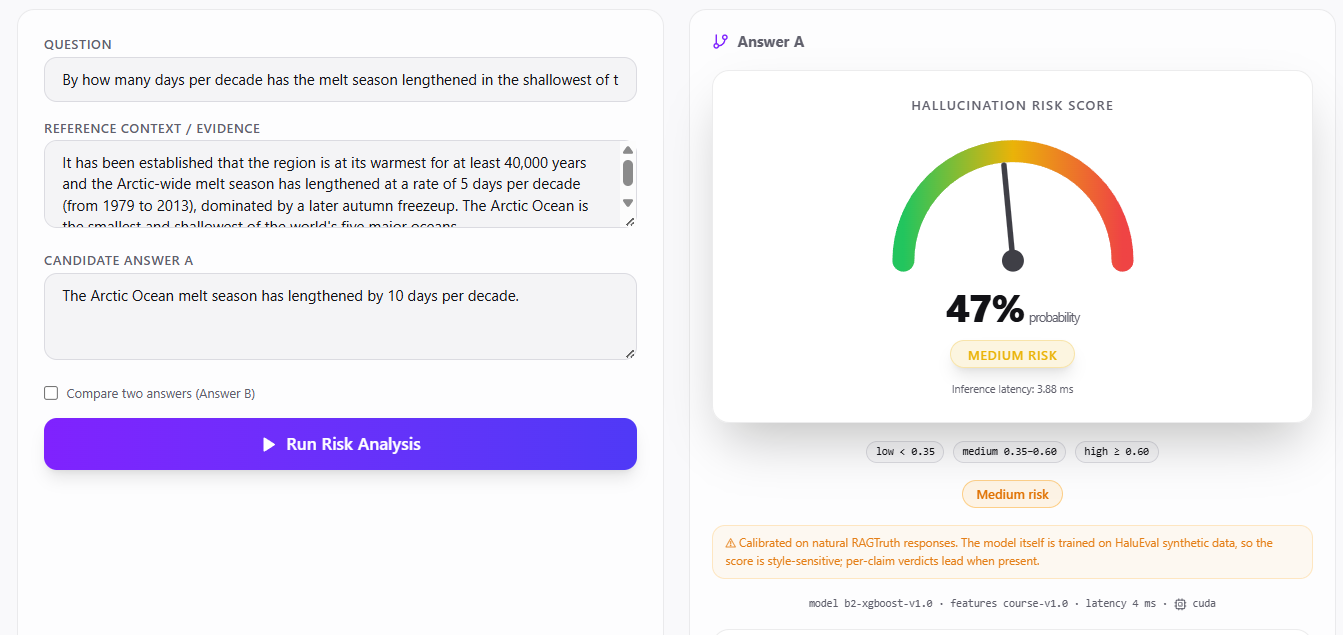
\includegraphics[width=\linewidth]{hallucinated_date.png}
    \caption{Hallucinated number: evidence-domain score 0.47}
  \end{subfigure}\hfill
  \begin{subfigure}[t]{0.40\linewidth}
    \centering
    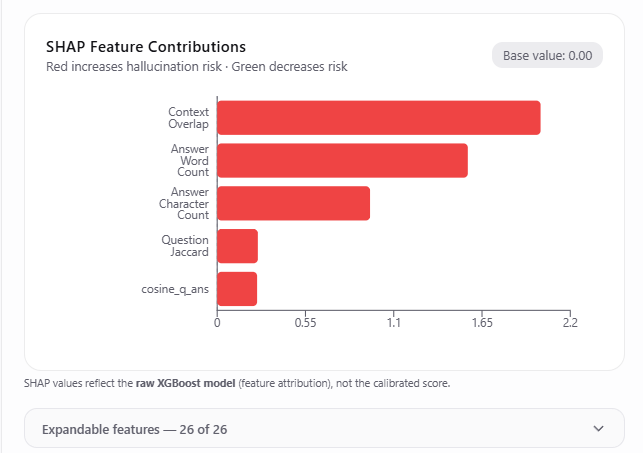
\includegraphics[width=\linewidth]{hallucinated_shap.png}
    \caption{SHAP contributions, hallucinated}
  \end{subfigure}
  \\[0.8em]
  \begin{subfigure}[t]{0.58\linewidth}
    \centering
    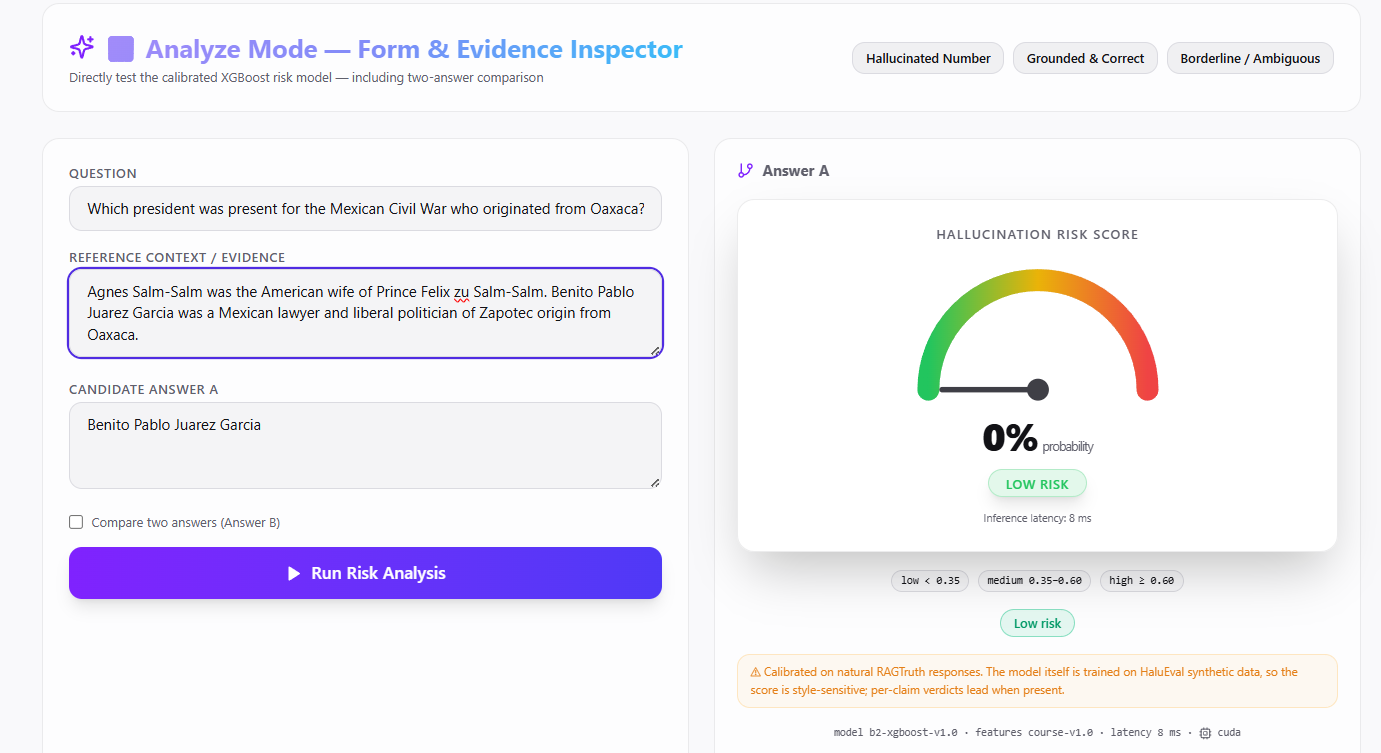
\includegraphics[width=\linewidth]{grounded_correct.png}
    \caption{Grounded: score below 0.01}
  \end{subfigure}\hfill
  \begin{subfigure}[t]{0.40\linewidth}
    \centering
    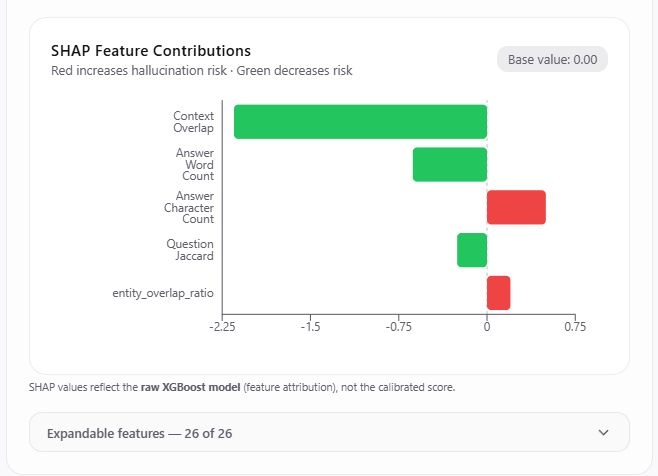
\includegraphics[width=\linewidth]{ground_shap.png}
    \caption{SHAP contributions, grounded}
  \end{subfigure}
  \caption{Analyze page cases with the raw-model SHAP contribution charts. Top: a hallucinated number, where the context states 5 days per decade and the answer states 10. Bottom: a grounded answer.}
  \label{fig:screens}
\end{figure}

\subsection{Reproducibility}

The source repository contains the complete pipeline. \texttt{src/data} holds the download and split scripts, \texttt{src/features} the seven feature groups, \texttt{src/models} the training protocol together with the cross-domain, calibration-shift, and explanation-reliability runs, \texttt{src/explain} the SHAP analysis, and \texttt{src/api} the FastAPI application. \texttt{requirements.txt} pins every dependency with exact versions. The train, validation, and test split indices are saved to \texttt{artifacts/split\_indices.json} and \texttt{.npy}, all seeds are centralized in the run configuration, and the model, calibrator, scaler, and SHAP explainer artifacts are stored under \texttt{artifacts/models/}.

The full experiment protocol is reproducible end to end. A self-contained Colab notebook (\texttt{colab/HaluRISC\_Training\_Version\_B.ipynb}) embeds the runtime source, verifies file hashes before execution, runs the pipeline on a GPU, and persists the artifacts to Google Drive. The \texttt{run\_all\_experiments.py} script reproduces the B-run locally from a frozen configuration (\texttt{configs/version\_b.yaml}), \texttt{make\_manifest.py} freezes the artifact hashes into \texttt{manifest.frozen.json}, and \texttt{verify\_artifacts.py} checks that every reported number matches the frozen artifacts. The manuscript itself is built from the same files that the dashboard reads, so the tables in Section~\ref{sec:results} trace back to the artifact files, including the length-binned error table and the reviewed audit sheet.

The environment is Python 3.12 on Windows 11 with an NVIDIA RTX 3060 6\,GB GPU (CUDA 12.8, torch 2.11.0+cu128) and 32\,GB of RAM, using scikit-learn 1.9.0, XGBoost 3.3.0, SHAP 0.52.0, spaCy 3.8.14, and sentence-transformers 5.6.1. The frontend uses Next.js 16.3.0 with pnpm.

\section{Experiment}\label{sec:experiment}

\subsection{Dataset}

The QA subset of HaluEval \cite{haluEval} is the training source. It contains 10{,}000 questions, each with a knowledge passage, a correct answer, and a hallucinated answer, which gives 20{,}000 labeled rows. The rows are split 70/15/15 at the question-group level, producing 14{,}000 training, 3{,}000 validation, and 3{,}000 test rows. This grouped, leakage-free design matters because both answer variants of a question share the same context, and a random split could otherwise let the model memorize the pairing. The split indices are saved for exact reproducibility.

Transfer is measured on RAGTruth \cite{ragtruth}, a corpus of naturally generated responses with human word-level span annotations, and on FaithBench \cite{faithbench}, a summarization hallucination benchmark built from modern LLM outputs. The RAGTruth QA task contributes 5{,}934 rows in 989 groups, of which 5{,}034 rows (839 groups) form the recalibration set and 900 rows (150 groups) the held-out test, with no overlapping groups between the two. Table~\ref{tab:datasets} summarizes the corpora.

\begin{table}[pos=htbp]
  \centering
  \caption{Datasets used for training and evaluation.}
  \label{tab:datasets}
  \begin{tabular}{|l|c|c|c|}
    \hline
    \textbf{Corpus} & \textbf{Rows} & \textbf{Groups} & \textbf{Use}              \\
    \hline
    HaluEval QA     & 20{,}000      & 10{,}000        & train / validation / test \\
    \hline
    RAGTruth QA     & 5{,}934       & 989             & zero-shot + recalibration \\
    \hline
    RAGTruth full   & 17{,}790      & 2{,}965         & zero-shot                 \\
    \hline
    FaithBench      & 750           & 750             & zero-shot                 \\
    \hline
  \end{tabular}
\end{table}

Text is whitespace-normalized. Lexical features operate on lowercased token sets, while NER and NLI keep the original casing. Missing context is handled explicitly, with lexical overlap set to zero and NLI probabilities to one third. All three corpora are used under their original licenses: HaluEval and RAGTruth are MIT-licensed, and FaithBench is distributed under CC BY-NC-SA 4.0. Raw files are not redistributed. The repository ships the download scripts, source revisions, and SHA-256 hashes instead, so every split can be regenerated from the original repositories.

\subsection{Evaluation Protocol}

Models are compared on precision, recall, F1, AUROC, PR-AUC, and MCC, and calibration with expected calibration error over 10 bins, Brier score, and negative log-likelihood. Hyperparameters are chosen by a randomized search of 30 iterations with grouped 5-fold cross-validation on the training split. Every experiment is repeated with seeds 42, 123, and 456 and reported as the mean over seeds. Significance is assessed with McNemar's test on paired test predictions, bootstrap 95\% confidence intervals from 1{,}000 resamples, and a Wilcoxon signed-rank test across seeds. The group structure is respected everywhere, so the two rows of one question never appear in both the training and the evaluation folds.

\subsection{Calibration Protocol}

Calibrators are fit on the validation split only, and the comparison of raw, Platt-scaled, and isotonic probabilities happens on the test split. The target-domain protocol follows the same principle. The recalibration set of 5{,}034 RAGTruth QA rows is used only to fit the target calibrator, and all reported numbers come from the disjoint 900-row test set.

\subsection{Explainability Protocol}

Global explanations come from a SHAP TreeExplainer \cite{shap} over the raw XGBoost model. Three measurements check whether the explanations are trustworthy. First, the mean absolute SHAP ranking is compared against permutation importance with a Kendall tau correlation. Second, the top-5 feature set is re-estimated from 1{,}000 bootstrap resamples and compared with the Jaccard index. Third, two perturbation studies are run on the test answers. Content edits replace entities, numbers, or dates, remove the supporting context, or insert an irrelevant sentence, and each edit should move the calibrated score if it changes the evidence. Structure edits shuffle the clause order, and these should leave the score nearly unchanged. For each operator the mean absolute score change, the fraction of large score changes, the top-1 SHAP flip rate, and the Spearman correlation between the original and perturbed scores are recorded. A neutralization study sets the top-$k$ SHAP features of each sample to its median and tracks the mean score change for $k = 1, 3, 5, 10$.

\subsection{Efficiency and Judge Protocol}

Latency is measured on 200 test samples on the reference laptop with an RTX 3060 6\,GB GPU, where NLI and embeddings run on the GPU and the remaining features on the CPU. The LLM-as-judge comparison uses GPT 5.6 Luna on the same 200 samples with a fixed prompt, and the cost is computed from the recorded token counts.

\section{Results}\label{sec:results}

\subsection{Model comparison}

Table~\ref{tab:models} reports the test-set performance of every baseline, averaged over the three seeds. XGBoost reaches an F1 of 0.9846 with an AUROC of 0.9979, ahead of the random forest by 0.0004 in F1 and the logistic regression by 0.0186. The overlap heuristic, which needs no training beyond its threshold, still reaches an F1 of 0.9352, and a majority baseline that predicts the negative class for everything scores zero, which confirms that the labels are balanced. The NLI-only baseline lags at 0.6714, which shows that the lexical, length, and semantic signals carry information the NLI cross-encoder alone does not. The TF-IDF variants sit between these extremes, with an answer-only linear model at 0.9224 and a full-input model at 0.5999. The margin between XGBoost and the random forest is small but significant in a McNemar test on the paired test predictions ($p = 0.044$), while the comparison against logistic regression ($p = 0.43$) and the heuristic ($p = 0.35$) is not significant. The Wilcoxon test across the three seeds finds no difference, which is expected given that the test compares only three points. Bootstrap confidence intervals for XGBoost are F1 $[0.9812,\,0.9895]$ and AUROC $[0.9964,\,0.9989]$.

The split design is verified against a known confound. A row-level split, where the two rows of one question can fall into different partitions, inflates F1 to 0.9886, and the grouped split corrects this to 0.9846, a drop of 0.004 in F1 and 0.0001 in AUROC. The reported numbers all use the grouped split, so the margin is small but real.

\begin{table}[pos=htbp]
  \centering
  \caption{Test-set performance on HaluEval QA, mean over seeds 42/123/456 (n = 3{,}000). The ECE and Brier columns measure the reliability of each model's risk score.}
  \label{tab:models}
  \footnotesize
  \setlength{\tabcolsep}{3.5pt}
  \begin{tabular}{|l|r|r|r|r|r|r|r|r|}
    \hline
    \textbf{Model}          & \textbf{P} & \textbf{R} & \textbf{F1} & \textbf{AUROC} & \textbf{PR-AUC} & \textbf{MCC} & \textbf{ECE} & \textbf{Brier} \\
    \hline
    Heuristic (1$-$overlap) & 0.947      & 0.923      & 0.935       & 0.913          & 0.820           & 0.872        & 0.354        & 0.267          \\
    \hline
    Logistic regression     & 0.977      & 0.955      & 0.966       & 0.993          & 0.990           & 0.933        & 0.010        & 0.025          \\
    \hline
    Random forest           & 0.990      & 0.979      & 0.984       & 0.998          & 0.998           & 0.969        & 0.014        & 0.013          \\
    \hline
    NLI-only                & 0.648      & 0.697      & 0.671       & 0.718          & 0.753           & 0.319        & 0.068        & 0.218          \\
    \hline
    TF-IDF (answer-only)    & 0.955      & 0.892      & 0.922       & 0.970          & 0.967           & 0.852        & 0.083        & 0.066          \\
    \hline
    TF-IDF (full input)     & 0.640      & 0.565      & 0.600       & 0.675          & 0.679           & 0.248        & 0.068        & 0.233          \\
    \hline
    XGBoost (standard)      & 0.993      & 0.976      & 0.985       & 0.998          & 0.998           & 0.970        & 0.004        & 0.012          \\
    \hline
  \end{tabular}
\end{table}

Single-answer behavior is worth one more look, since the models disagree in ways that aggregate metrics hide. For a grounded span and a hallucinated sentence that share one question and one context, the overlap heuristic and the NLI-only model fail to separate the pair (0.0000 against 0.0769 and 0.3928 against 0.3950), and the answer-only TF-IDF model puts the grounded span at 0.7490 while flagging the hallucinated case at 0.9121. Logistic regression, random forest, and XGBoost separate the pair cleanly. A third case, a grounded one-word answer, is flagged by the heuristic, logistic regression, the random forest, and the raw XGBoost, and the deployed calibrator maps those raw probabilities to 0.0000, which is why the system displays the calibrated score and keeps the raw score as a secondary signal.

\subsection{Evidence-consistent XGBoost}

Table~\ref{tab:ec} reports the component ablation for EC-XGB on the HaluEval test set, averaged over the three seeds. The standard XGBoost reference (m0) reaches an F1 of 0.9844, the length debias and monotone constraints (m1) reach 0.9852, the claim-level aggregates (m2) reach 0.9857, and the full EC-XGB (m3) reaches 0.9858 with an MCC of 0.9719. The differences are small and not significant in a McNemar test on the paired predictions (m0 against m3, $p = 0.63$), and a Wilcoxon test across seeds finds no difference either ($p = 0.25$). The benchmark is saturated, so this ablation is a preservation check rather than a win. Every component holds the line, and the false-alarm count improves slightly: on the seed-42 test split the standard model makes 12 false positives and EC-XGB makes 8.

\begin{table}[pos=htbp]
  \centering
  \caption{EC-XGB component ablation on the HaluEval test set, mean over seeds 42/123/456 (n = 3{,}000). m0 is the standard XGBoost reference, m1 adds log-scaled length features and monotone constraints, m2 adds the claim-level aggregates, and m3 is the deployed EC-XGB.}
  \label{tab:ec}
  \footnotesize
  \setlength{\tabcolsep}{5pt}
  \begin{tabular}{|l|c|c|c|c|c|}
    \hline
    \textbf{Variant} & \textbf{Features} & \textbf{F1} & \textbf{AUROC} & \textbf{MCC} & \textbf{ECE} \\
    \hline
    m0 standard  & 26 & 0.9844 & 0.9980 & 0.9693 & 0.0066 \\
    \hline
    m1 debias    & 26 & 0.9852 & 0.9976 & 0.9708 & 0.0051 \\
    \hline
    m2 + claims  & 34 & 0.9857 & 0.9984 & 0.9717 & 0.0068 \\
    \hline
    m3 EC-XGB    & 35 & 0.9858 & 0.9985 & 0.9719 & 0.0078 \\
    \hline
  \end{tabular}
\end{table}

Table~\ref{tab:shift} shows where the modification matters. Every model is applied without retraining to the RAGTruth and FaithBench corpora. The standard model flags almost every natural answer as risky, since 99.9\% of RAGTruth rows and 99.5\% of FaithBench rows cross the 0.5 threshold, which makes the decision rule useless outside the benchmark even though recall stays high. EC-XGB cuts the flag rate to 61.3\% on the RAGTruth test tasks and to 7.2\% on FaithBench, raises the AUROC from 0.475 to 0.573 and from 0.509 to 0.587, and lowers the ECE on RAGTruth from 0.635 to 0.283. The held-out RAGTruth QA task is the strictest test, since its rows never enter training. There the F1 stays flat (0.3022 against 0.3069) and the ECE improves from 0.815 to 0.756, which shows that multi-source training does not transfer a new task for free. On FaithBench the conservative regime lowers the F1 from 0.813 to 0.119. The standard model earns that F1 by flagging nearly every row, so the AUROC and the flag rate are the fair comparison at this operating point, and the F1 drop is reported as a limitation rather than hidden.

\begin{table}[pos=htbp]
  \centering
  \caption{Zero-shot shift behavior, mean over seeds. Standard is the B2 XGBoost trained on HaluEval only. EC-XGB adds the RAGTruth non-QA training rows. Flagged is the share of rows above the 0.5 threshold, and the RAGTruth QA rows never enter training.}
  \label{tab:shift}
  \footnotesize
  \setlength{\tabcolsep}{4.5pt}
  \begin{tabular}{|l|l|c|c|c|c|}
    \hline
    \textbf{Corpus} & \textbf{Model} & \textbf{F1} & \textbf{AUROC} & \textbf{Flagged} & \textbf{ECE} \\
    \hline
    RAGTruth all & Standard & 0.5181 & 0.4753 & 99.9\% & 0.6346 \\
    \hline
    RAGTruth all & EC-XGB   & 0.5632 & 0.5731 & 61.3\% & 0.2827 \\
    \hline
    RAGTruth QA  & Standard & 0.3022 & 0.5465 & 99.9\% & 0.8149 \\
    \hline
    RAGTruth QA  & EC-XGB   & 0.3069 & 0.5352 & 98.1\% & 0.7555 \\
    \hline
    FaithBench   & Standard & 0.8130 & 0.5089 & 99.5\% & 0.2917 \\
    \hline
    FaithBench   & EC-XGB   & 0.1192 & 0.5866 & 7.2\%  & 0.4512 \\
    \hline
  \end{tabular}
\end{table}

The operating-point mode selects the threshold on the HaluEval validation split that maximizes recall under a five percent false-positive budget. Across the three seeds the test false-positive rate lands between 4.2\% and 5.1\% while the test recall stays between 99.0\% and 99.5\%, which gives a deployment option for recall-first users at a cost of about one point of F1. For the deployed display score, a Platt calibrator fitted on the 5{,}034-row RAGTruth QA calibration split reduces the ECE on the held-out 900-row QA test from 0.735 to 0.126, close to the 0.1335 reached by target recalibration of the standard model.

\subsection{Calibration on the source domain}

Table~\ref{tab:calib} compares raw, Platt-scaled, and isotonic probabilities on the HaluEval test set. The raw model is already well calibrated with an ECE of 0.0045, and neither recalibration improves it, since Platt raises the ECE to 0.0091 and isotonic to 0.0070. This is an honest negative result: the logistic objective already produces reliable probabilities on this benchmark, and the reliability diagrams in Figure~\ref{fig:reliability} confirm that the raw curve tracks the diagonal.

\begin{table}[pos=htbp]
  \centering
  \caption{Calibration on the HaluEval test set (mean over seeds).}
  \label{tab:calib}
  \begin{tabular}{|l|r|r|r|r|}
    \hline
    \textbf{Method} & \textbf{F1} & \textbf{ECE} & \textbf{Brier} & \textbf{NLL} \\
    \hline
    Raw XGBoost     & 0.985       & 0.0045       & 0.0117         & 0.045        \\
    \hline
    Platt (sigmoid) & 0.985       & 0.0091       & 0.0129         & 0.058        \\
    \hline
    Isotonic        & 0.984       & 0.0070       & 0.0124         & 0.073        \\
    \hline
  \end{tabular}
\end{table}

\begin{figure}[pos=htbp]
  \centering
  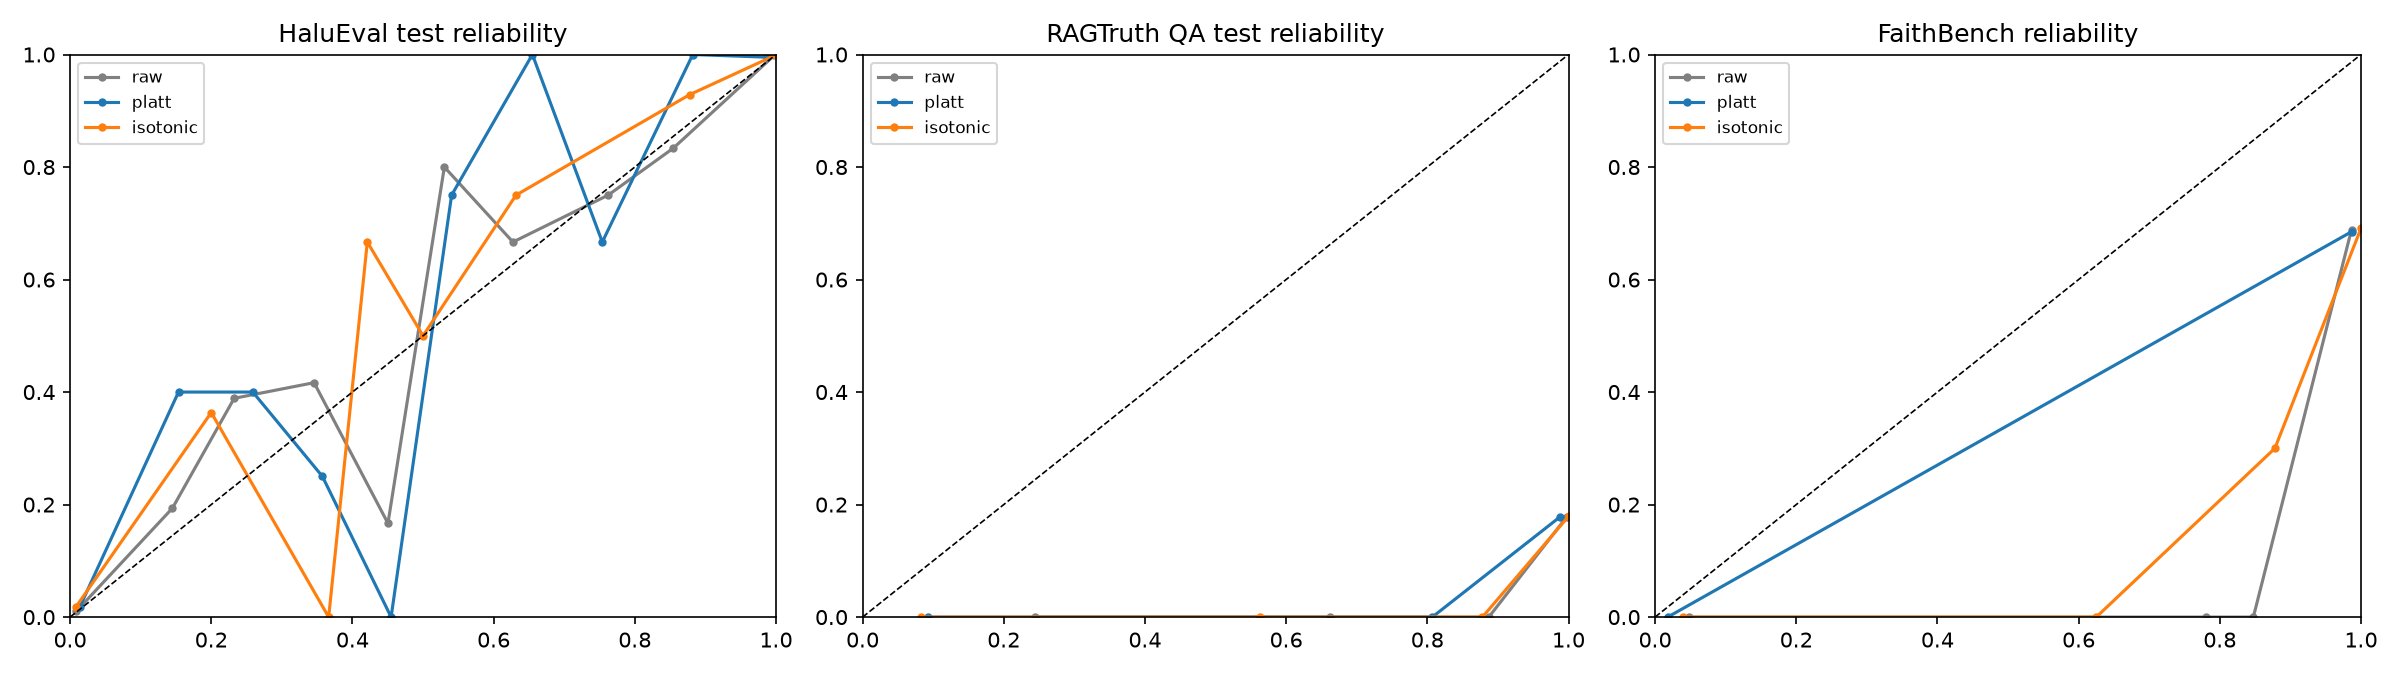
\includegraphics[width=0.8\linewidth]{b4/reliability_diagrams.png}
  \caption{Reliability diagrams of the raw, Platt-calibrated, and isotonic models on the HaluEval test set (left), RAGTruth QA (middle), and FaithBench (right).}
  \label{fig:reliability}
\end{figure}

\subsection{Target-domain recalibration}

Table~\ref{tab:target} applies the standard model to the 900-row RAGTruth QA test set and compares raw scores, the source calibrator fitted on the HaluEval validation split, and calibrators re-fitted on 5{,}034 RAGTruth rows. The raw and source-calibrated probabilities are badly off, with an ECE above 0.8, and target recalibration cuts the ECE to 0.1335 (Platt) and 0.1316 (isotonic) and the Brier score from 0.801 to 0.164. One deployment caveat is visible in the same numbers: the predicted positive rate drops to nearly zero at the fixed 0.5 threshold, so a deployment must also retune the decision threshold, and the labels follow only after that second step.

\begin{table}[pos=htbp]
  \centering
  \caption{Target-domain recalibration on RAGTruth QA (calibration n = 5{,}034, test n = 900).}
  \label{tab:target}
  \begin{tabular}{|l|r|r|r|r|}
    \hline
    \textbf{Calibrator}     & \textbf{ECE} & \textbf{Brier} & \textbf{NLL} & \textbf{Pred. pos.} \\
    \hline
    Raw scores              & 0.8185       & 0.8164         & 5.20         & 0.999               \\
    \hline
    Source Platt (HaluEval) & 0.8089       & 0.8011         & 3.62         & 0.999               \\
    \hline
    Target Platt (RAGTruth) & 0.1335       & 0.1639         & 0.51         & 0.000               \\
    \hline
    Target isotonic         & 0.1316       & 0.1663         & 0.53         & 0.000               \\
    \hline
  \end{tabular}
\end{table}

\begin{figure}[pos=htbp]
  \centering
  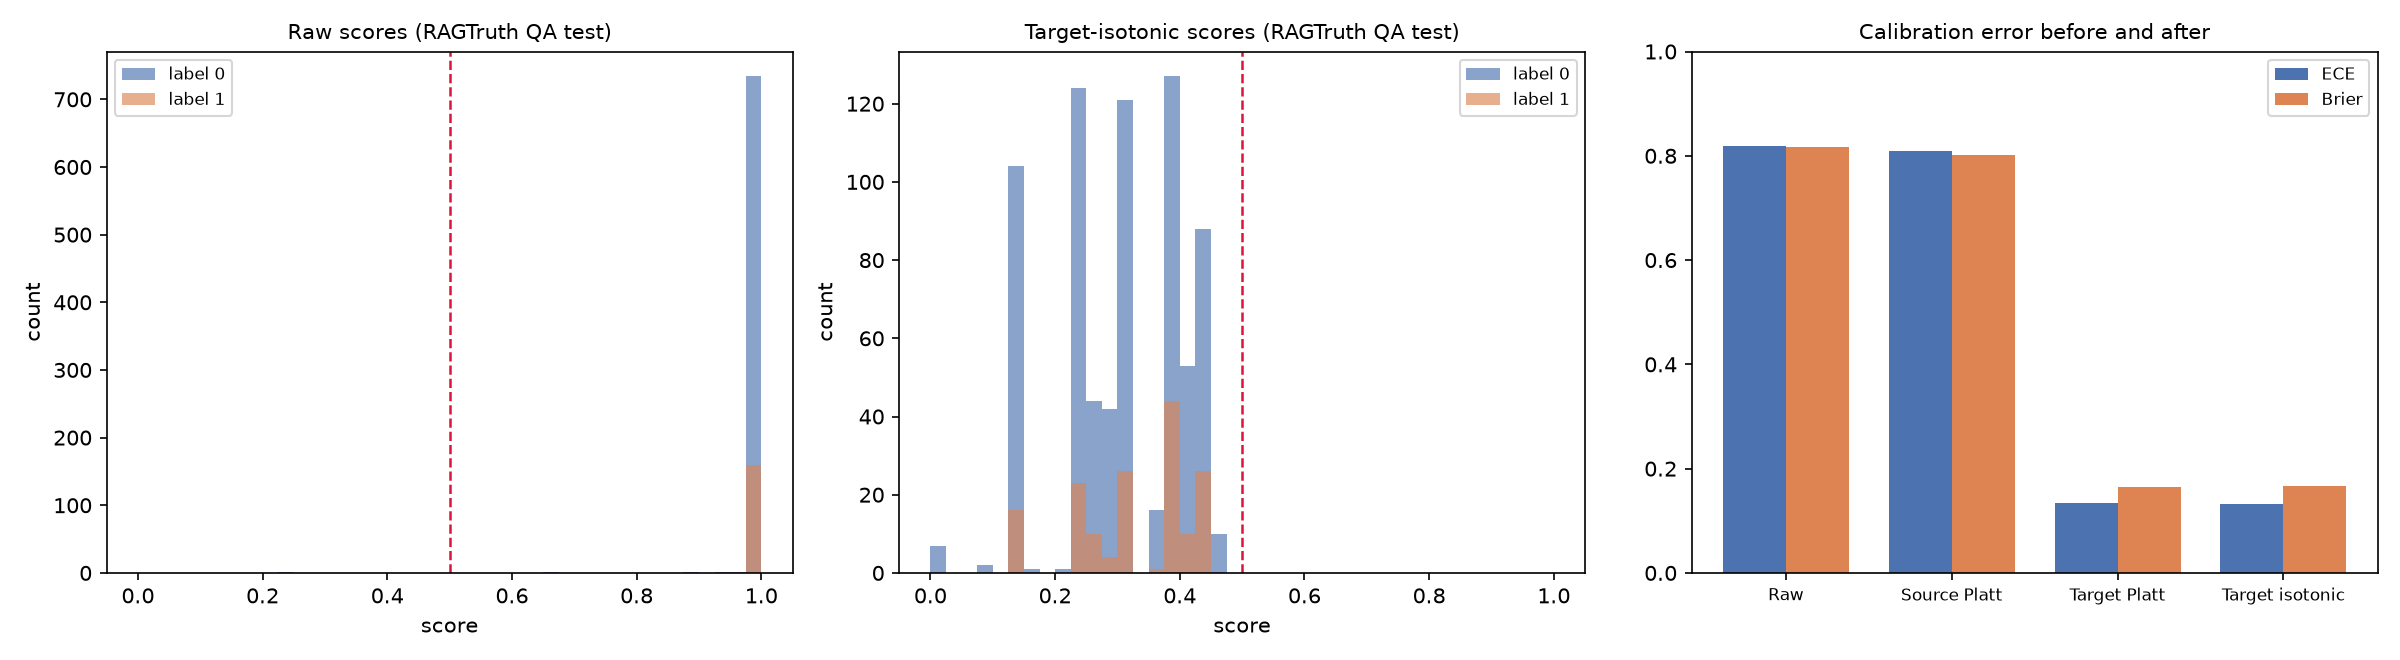
\includegraphics[width=0.8\linewidth]{b4/calibration_shift.png}
  \caption{Target-domain recalibration on RAGTruth QA. Left and middle: raw and target-calibrated score distributions on the 900-row test set, with the 0.5 threshold marked. Right: ECE and Brier before and after recalibration.}
  \label{fig:calibshift}
\end{figure}

\subsection{Cross-domain zero-shot transfer}

The zero-shot evaluation with no training or adaptation on the target corpora is the central negative result of the paper. On the 900-row RAGTruth QA split the standard model reaches an F1 of 0.302, an AUROC of 0.540, a PR-AUC of 0.190, an MCC of 0.016, and an ECE of 0.819, and the recall is 1.0 on every corpus: the model flags almost everything, the precision lands on the label prior, and the AUROC stays near 0.5. Synthetic HaluEval hallucinations differ systematically from naturally generated responses. FaithBench sits between the two extremes at an F1 of 0.8130 and an AUROC of 0.5314, since its summaries are shorter and closer to the HaluEval format, and the combined RAGTruth set lands at an F1 of 0.603, an AUROC of 0.497, and an ECE of 0.560. The RAGTruth task breakdown repeats the pattern, with F1 of 0.4515 on QA, 0.4603 on summarization, and 0.8140 on data-to-text, and the F1 rises from 0.4940 on very short contexts to 0.7091 on contexts with 128 to 511 characters. Figure~\ref{fig:transferscore} plots the score distributions behind these numbers.

\begin{figure}[pos=htbp]
  \centering
  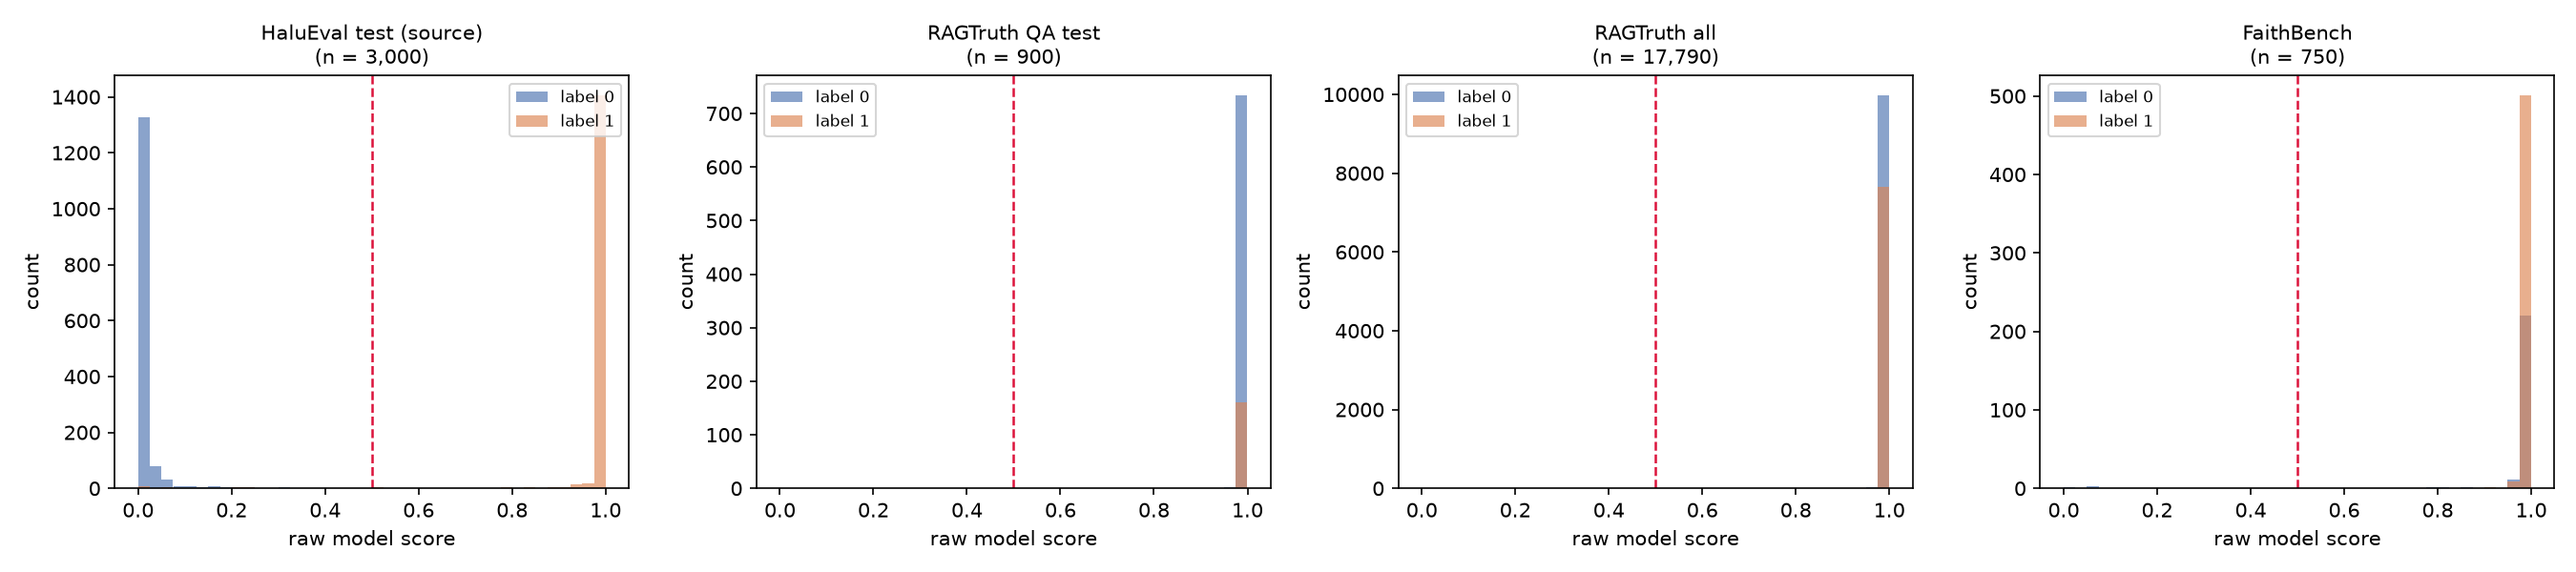
\includegraphics[width=0.8\linewidth]{b3/transfer_score_distributions.png}
  \caption{Raw model score distributions on the HaluEval test set and the zero-shot corpora, with the 0.5 threshold marked. The source panel separates the classes, while every zero-shot panel piles both labels at 1.0.}
  \label{fig:transferscore}
\end{figure}

\subsection{Ablation}

Table~\ref{tab:ablation} removes each feature group and retrains from scratch with the same protocol. Lexical features dominate, with the F1 dropping by 0.0247 when they are removed, while length and NLI contribute smaller amounts and the entity, numeric, and hedging groups stay neutral within 0.0002. Removing the semantic group slightly improves the F1, a negative result reported rather than hidden, and the ranking agrees with the SHAP analysis next.

\begin{table}[pos=htbp]
  \centering
  \caption{Feature-group ablation, mean over seeds (full model F1 = 0.9846, AUROC = 0.9979).}
  \label{tab:ablation}
  \begin{tabular}{|l|r|r|r|}
    \hline
    \textbf{Removed group} & \textbf{F1} & \textbf{$\Delta$F1} & \textbf{AUROC} \\
    \hline
    length                 & 0.9801      & $-$0.0045           & 0.9963         \\
    \hline
    lexical                & 0.9600      & $-$0.0247           & 0.9923         \\
    \hline
    entity                 & 0.9847      & $+$0.0001           & 0.9982         \\
    \hline
    nli                    & 0.9823      & $-$0.0023           & 0.9973         \\
    \hline
    numeric                & 0.9844      & $-$0.0002           & 0.9982         \\
    \hline
    hedging                & 0.9848      & $+$0.0001           & 0.9981         \\
    \hline
    semantic               & 0.9860      & $+$0.0014           & 0.9982         \\
    \hline
  \end{tabular}
\end{table}

\subsection{Explanation reliability}

Figure~\ref{fig:shapimp} shows the mean absolute SHAP values for the top-12 features. The context overlap dominates, followed by the answer length features, the context-to-answer contradiction probability, and the question-to-answer cosine. The explanation set agrees with the ablation in spirit, since lexical and length features carry the largest weights. Three checks assess whether the explanations are stable. The SHAP ranking agrees with permutation importance at a Kendall tau of 0.66. The top-5 feature set is identical across 1{,}000 bootstrap resamples, with a Jaccard of 1.0. Neutralizing the top-$k$ features drops the mean score monotonically from $-$0.079 at $k=1$ to $-$0.412 at $k=10$, which confirms that the top features are actually driving the predictions rather than decorating them.

Table~\ref{tab:perturb} reports the perturbation study. Content edits move the score in proportion to the semantic weight of the edit. Replacing an entity changes the score by 0.360 on average, a number by 0.345, a date by 0.279, and removing the supporting context by 0.272. The irrelevant insert and clause shuffle leave the score nearly untouched, at 0.006 and 0.001. The top-1 SHAP feature never flips under any operator, and the Spearman correlation stays between 0.84 and 0.95. The sample sizes are small for dates and clause shuffles, 13 and 14 respectively, because not every answer contains an edit-able element, and the table reports n openly.

\begin{table}[pos=htbp]
  \centering
  \caption{Perturbation stability of the calibrated score and SHAP ranking.}
  \label{tab:perturb}
  \begin{tabular}{|l|c|r|r|r|r|}
    \hline
    \textbf{Operator}  & \textbf{n} & \textbf{$\Delta$score} & \textbf{Large rate} & \textbf{Top-1 flip} & \textbf{Spearman} \\
    \hline
    Entity replacement & 78         & 0.360                  & 0.372               & 0.000               & 0.840             \\
    \hline
    Number replacement & 22         & 0.345                  & 0.364               & 0.000               & 0.852             \\
    \hline
    Date replacement   & 13         & 0.279                  & 0.308               & 0.000               & 0.870             \\
    \hline
    Support removal    & 66         & 0.272                  & 0.288               & 0.000               & 0.874             \\
    \hline
    Irrelevant insert  & 120        & 0.006                  & 0.008               & 0.000               & 0.948             \\
    \hline
    Clause shuffle     & 14         & 0.001                  & 0.000               & 0.000               & 0.921             \\
    \hline
  \end{tabular}
\end{table}

\begin{figure}[pos=htbp]
  \centering
  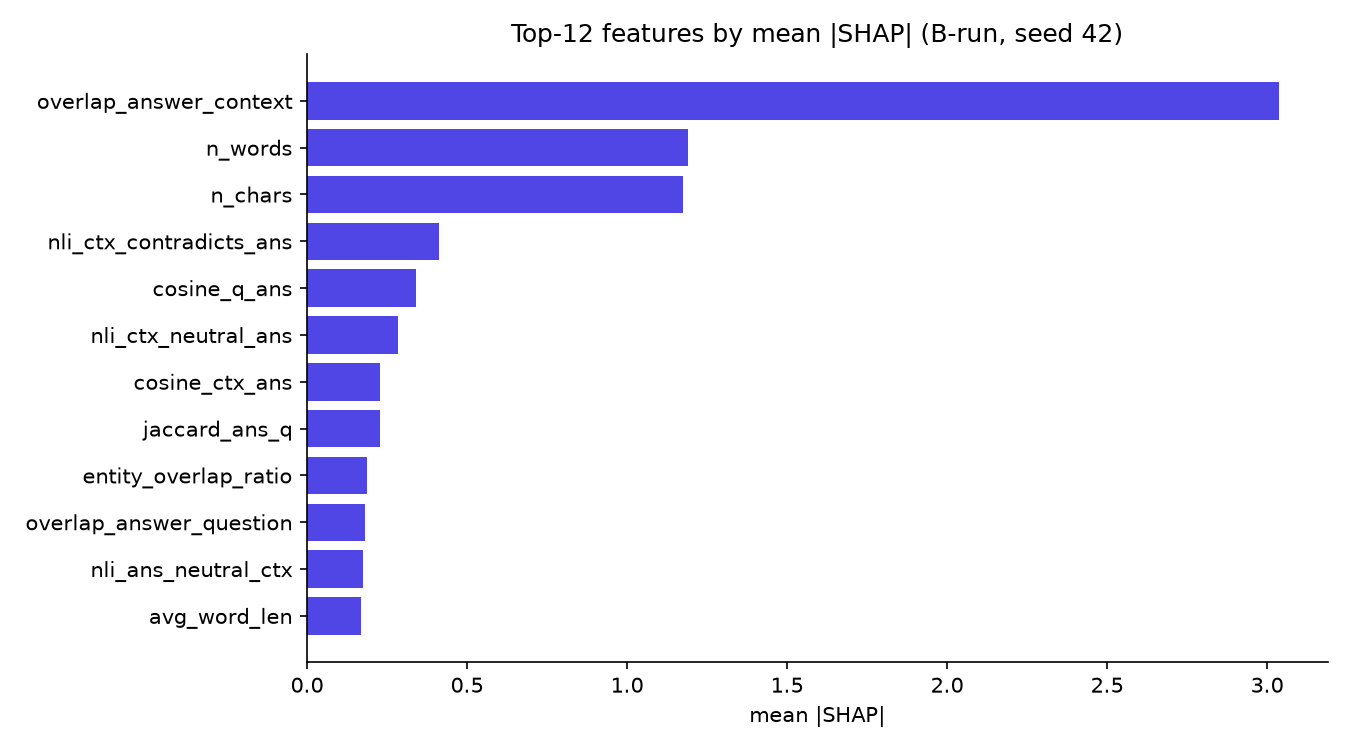
\includegraphics[width=0.8\linewidth]{fig_shap_importance_b5.png}
  \caption{Mean absolute SHAP values for the top-12 features (B-run, seed 42).}
  \label{fig:shapimp}
\end{figure}

A structured expert audit tested these explanations case by case. The B5 run exported 26 error-enriched cases (9 false positives, 10 false negatives, and 7 inside the 0.35 to 0.65 band), and two review passes were performed with an AI assistant, which the released sheet records in a review-mode field. Both passes judged the explanation against the answer-context evidence rather than the dataset label, they agreed on 23 of 26 cases (88\%), and both marked 15 cases implausible. The three disagreements all sit on borderline scores. False positives inherit the length confound of the benchmark, and false negatives occur when a wrong answer reuses entities that appear in the context, which keeps lexical overlap high. Two audited cases (items 2251 and 2436) carry a hallucinated label even though the context directly supports the answer, so they look like benchmark label noise rather than model errors. The audit sample is deliberately error-heavy, so these proportions describe the audit and not the test set.

\subsection{Efficiency and cost}

Table~\ref{tab:latency} breaks down the latency over 200 test samples. The NLI cross-encoder and the spaCy entity pass dominate at 27.1\,ms and 21.1\,ms median, while the model itself needs 1.3\,ms and SHAP 1.9\,ms. The total is 61.8\,ms at the median, the deployed artifact weighs 0.82\,MB, and the marginal cost of a local prediction is about \$0.001 per 1{,}000 calls.

\begin{table}[pos=htbp]
  \centering
  \caption{Per-component latency in ms (n = 200).}
  \label{tab:latency}
  \begin{tabular}{|l|r|r|r|}
    \hline
    \textbf{Component} & \textbf{p50} & \textbf{p95} & \textbf{mean} \\
    \hline
    Core lexical       & 0.10         & 0.15         & 0.11          \\
    \hline
    Entity (spaCy NER) & 21.13        & 47.24        & 25.34         \\
    \hline
    NLI (2 directions) & 27.09        & 68.60        & 40.09         \\
    \hline
    Semantic (MiniLM)  & 9.25         & 15.55        & 12.56         \\
    \hline
    XGBoost inference  & 1.26         & 8.80         & 2.62          \\
    \hline
    SHAP explanation   & 1.91         & 15.52        & 3.65          \\
    \hline
    Total per sample   & 61.77        &              &               \\
    \hline
  \end{tabular}
\end{table}

\subsection{LLM-as-judge comparison}

Table~\ref{tab:judge} compares the deployed model with GPT 5.6 Luna on the same 200 samples. The judge reaches an F1 of 0.841 against 0.985 for the model, the two agree on 84.5\% of the cases, and the paired McNemar test is highly significant ($p = 1.6 \times 10^{-5}$), with 28 cases where the judge is wrong and the model is right against 3 where the roles are reversed. The judge costs \$0.105 per 1{,}000 predictions and needs 1.3 seconds at the median, while the model costs about \$0.001 per 1{,}000 and runs in 61.8\,ms.

\begin{table}[pos=htbp]
  \centering
  \caption{LLM-as-judge vs.\ XGBoost on 200 test samples.}
  \label{tab:judge}
  \begin{tabular}{|l|r|r|r|r|r|r|}
    \hline
    \textbf{Model}     & \textbf{Acc} & \textbf{P} & \textbf{R} & \textbf{F1} & \textbf{p50 (ms)} & \textbf{Cost/1K} \\
    \hline
    GPT 5.6 Luna judge & 0.860        & 0.974      & 0.740      & 0.841       & 1310              & \$0.105          \\
    \hline
    XGBoost (ours)     & 0.985        & 0.980      & 0.990      & 0.985       & 62                & $\approx$\$0.001 \\
    \hline
  \end{tabular}
\end{table}

\subsection{Error analysis}

The 3{,}000-sample test set contains 48 errors, 12 false positives and 36 false negatives, an error rate of 1.6\%. A manual inspection of 20 sampled errors assigns them to two categories. Short-answer ambiguity covers very short answers where neither the lexical nor the NLI evidence is decisive, and label ambiguity covers answers that are semantically plausible under both labels. Table~\ref{tab:errors} reports the counts. Both categories trace back to the construction of the benchmark, where short answers are frequently hallucinated by design.

\begin{table}[pos=htbp]
  \centering
  \caption{Error taxonomy for 20 sampled misclassifications.}
  \label{tab:errors}
  \begin{tabular}{|l|r|r|}
    \hline
    \textbf{Category}      & \textbf{FP} & \textbf{FN} \\
    \hline
    Label ambiguity        & 7           & 4           \\
    \hline
    Short-answer ambiguity & 3           & 6           \\
    \hline
  \end{tabular}
\end{table}

The length distribution behind those errors is the more informative signal. Table~\ref{tab:length} bins the full test set by answer length. The hallucinated share is 2.1\% among one-word answers and rises to 99.2\% above 17 words, so answer length is close to a perfect proxy for the label in HaluEval. The model reproduces the pattern: the mean score climbs from 0.024 to 0.993 across the bins, two-thirds of all false positives fall in the 5-8 word bin at a 10.6\% false-positive rate, and false negatives concentrate in the 1-4 word bins at about an 18\% rate. This mechanism explains the zero-shot transfer result. Natural RAGTruth responses are full sentences, so the model reads their length as evidence of hallucination, which is why recall reaches 1.0 and AUROC stays near 0.5 on that corpus. The deployed interface responds to this failure mode by leading with per-claim evidence verdicts and presenting the model score as a secondary signal.

\begin{table}[pos=htbp]
  \centering
  \caption{Test-set errors by answer length, mean over seeds (17+ contains only two negative rows).}
  \label{tab:length}
  \begin{tabular}{|l|r|r|r|r|r|}
    \hline
    \textbf{Words} & \textbf{Rows} & \textbf{Hallucinated} & \textbf{FP rate} & \textbf{FN rate} & \textbf{Mean score} \\
    \hline
    1              & 524           & 0.021                 & 0.004            & 0.182            & 0.024               \\
    \hline
    2              & 514           & 0.033                 & 0.000            & 0.176            & 0.035               \\
    \hline
    3--4           & 474           & 0.127                 & 0.002            & 0.178            & 0.126               \\
    \hline
    5--8           & 641           & 0.902                 & 0.106            & 0.031            & 0.888               \\
    \hline
    9--16          & 600           & 0.982                 & 0.000            & 0.003            & 0.980               \\
    \hline
    17+            & 247           & 0.992                 & 0.333            & 0.000            & 0.993               \\
    \hline
  \end{tabular}
\end{table}

\subsection{Discussion and limitations}

The results need to be read against multiple limitations. Around 85\% of HaluEval is generated with a sampling-then-filtering procedure \cite{bang-etal-2025-hallulens}, so its hallucination patterns are synthetic by construction, and the zero-shot transfer result on RAGTruth shows how far in-distribution performance is from natural responses. Length and overlap statistics are highly informative on HaluEval but may not carry over, as the ablation and SHAP analyses both indicate, and the binary benchmark label leaves graded severity and partially supported answers out of scope. The audit in Section~\ref{sec:results} found two cases where the hallucinated label contradicts the context, so a small amount of label noise remains. Every feature in the pipeline is English-centric, and the supervised model now trains on HaluEval plus the RAGTruth non-QA tasks, yet domain adaptation remains open work at this scale. Under domain shift EC-XGB trades recall for precision on unseen corpora, and the FaithBench result shows the cost, since the flag rate falls from 99.5\% to 7.2\% and the AUROC rises while the F1 drops because the model becomes conservative on a benchmark it never saw. The RAGTruth all-task gains also include task types that the multi-source training saw, so they measure adaptation rather than pure zero-shot transfer, and the held-out QA task improves mainly in calibration. On the source benchmark the raw probabilities are already well calibrated, while the EC-XGB display calibrator fitted on the RAGTruth QA split cuts the target ECE from 0.735 to 0.126. Finally, the calibrated score is style-sensitive in conversational use, since full-sentence answers can saturate it even when the per-claim evidence verdicts are supported, so the interface leads with the evidence verdicts and presents the model score as a secondary signal. Two established directions fit the verification layer next: RAGAs scores claim support and answer relevance without human review \cite{ragas2024}, and small verifier models make claim-level checks cheap enough for every answer \cite{minicheck2024}.

\subsection{Ethical considerations}

A hallucination-risk score predicts risk, not truth, and it must not be treated as a fact-checker. Over-reliance on automated detectors creates false trust, especially when scores are confidently wrong out of domain, which is exactly what the RAGTruth result demonstrates. Detection quality varies across domains and languages, and the current system is English-only. The interface therefore labels scores as risk estimates and shows a training-data warning with every prediction.

\section{Conclusion}\label{sec:conclusion}

Hallucination detection needs to be cheap, fast, and explainable before it is useful in practice. This study presented EC-XGB, an evidence-consistent XGBoost risk predictor that combines 26 engineered evidence-consistency features with eight claim-level NLI aggregates, log-scaled length features under monotone constraints, multi-source training, calibrated probabilities, and SHAP explanations. On HaluEval QA it reaches an F1 of 0.9858 and an AUROC of 0.9985, on par with the standard tuned XGBoost on a saturated benchmark, and it makes fewer false positives at the same operating point. The gain appears under domain shift, where the standard model flags 99.9\% of natural RAGTruth answers as risky and EC-XGB flags 61.3\%, with the AUROC rising from 0.475 to 0.573 and the ECE falling from 0.635 to 0.283. The deployed display calibrator cuts the RAGTruth QA ECE from 0.735 to 0.126. One analysis takes 61.8\,ms at the median and costs about \$0.001 per 1{,}000 predictions, roughly 100 times less than the GPT 5.6 Luna judge that it outperforms on the same 200 samples.

The negative results are reported with the same care as the positive ones. The raw model needs no recalibration on HaluEval, the entity and hedging features add no measurable value, and the held-out RAGTruth QA task stays near an F1 of 0.30 even after multi-source training, while the conservative FaithBench regime trades F1 for calibration. The paper therefore frames the supervised risk model as a benchmark and adaptation estimator, and the deployed system adds claim-level verification with evidence retrieval to cover the remaining transfer gap. Future work targets multicalibration under stronger shift, per-domain threshold transfer, and neural baselines for comparison.

%%% SECTION-INSERT-POINT %%%

\section*{Declarations}
\begin{itemize}
  \item \textbf{Conflicts of Interest:} The authors declare no conflicts of interest.

  \item \textbf{Data availability:} The raw evaluation corpora are not redistributed. The repository ships the download scripts, source revisions, SHA-256 hashes, and license notes for HaluEval (MIT), RAGTruth (MIT), and FaithBench (CC BY-NC-SA 4.0), so every split and feature matrix can be regenerated from the original sources. Model artifacts, split indices, and the frozen experiment manifest are included with the code release.

  \item \textbf{Code availability:} The training pipeline, FastAPI inference service, and Next.js dashboard are available in the project repository.
\end{itemize}
%%%%%%%%%%%%%%%%%%%%%%%%%%%%%%%
\printcredits

\bibliographystyle{elsarticle-num}
\bibliography{ref}

\vspace{12pt}
\end{document}
